\documentclass{beamer}
\usepackage[utf8]{inputenc}
\usepackage[T1]{fontenc}
\usepackage{tikz}
\usetheme{Warsaw}

\title[Le phantasme du jeu sans fin]{Le phantasme du jeu sans fin}
\author{Xavier Van de Woestyne}
\date{Avril 2014}
\begin{document}
\begin{frame}
\titlepage
\end{frame}

\AtBeginSection[]
{
  \begin{frame}{Plan}
  \begin{columns}[t]
  \begin{column}{5cm}
  \tableofcontents[sections={1-4},currentsection, currentsubsection,  hideothersubsections]
  \end{column}
  \begin{column}{5cm}
  \tableofcontents[sections={5-8},currentsection,currentsubsection, hideothersubsections]
  \end{column}
  \end{columns}
\end{frame}
}

\section{Introduction}

\subsection{Mise au point sur le thème}
\begin{frame}{Mise au point sur le thème}
  Je vous ai menti, je ne parlerai pas vraiment de la construction d'un jeu sans fin.\newline \newline
  \begin{itemize}
    \item Faire un jeu sans fin est très facile;
    \item Faire un jeu sans fin est probablement impossible.
  \end{itemize}
\end{frame}

\subsection{Contexte et motivations}
\begin{frame}{Contexte et motivations}
  \begin{itemize}
    \item Transversalité de deux passions;
    \item Curiosité;
    \item Envie de performance, recherche d'occupation.
  \end{itemize}
\end{frame}

\subsection{Méthodologie}
\begin{frame}{Méthodologie}
  \begin{itemize}
    \item Choix d'un genre (le J.R.P.G)
    \item Isolation de ce qui est important
    \item Formulation d'un postulat \\ 
      Ce qui fait qu'un jeu est jeu, c'est le jeu.
    \item Réflexion sur la découpe du jeu.
  \end{itemize}
\end{frame}

\section{Structure du jeu d'aventure}
\subsection{Quêtes}
\begin{frame}{Tout est quête}
Un dragon menace le monde, le héros doit le tuer. 
  \newline
  $$A \rightarrow B$$
  \begin{itemize}
    \item A : Situation intiale
    \item B : Situation finale (Dragon mort)
  \end{itemize}
\end{frame}

\subsection{Sous-quêtes et quêtes annexes}
\begin{frame}{Quêtes composées de quêtes}
  Une quête étant potentiellement composée.
  \newline
  $$A \rightarrow SQ_1 \rightarrow SQ_2 \rightarrow SQ_3 \rightarrow B $$
  \newline
  Une quête annexe étant une sous-quêtes s'extrayant de la dépendance relationnelle entre les autres quêtes.
\end{frame}

\subsection{La liste des quêtes est un  monoïde}
\begin{frame}{Liste de quêtes comme un monoïde}
  \begin{itemize}
    \item L'élément neutre est l'identité de la quête (non répétable, donc unique);
    \item Sa combinaison ($\oplus$): Empile une quête non-lancée avec un nouvel état;
    \item Les parenthèses n'agissent pas comme sous méthode de tri. (Associativité respectée).
  \end{itemize}
\end{frame}

\section{Usage de la littérature}
\subsection{Le structuralisme}
\begin{frame}{Un mot récurrent}
  \begin{center}
    \begin{block}{\textbf{Le structuralisme}}
      \textit{Etude des relations de transformation}
    \end{block}
  \end{center}
\end{frame}

\subsection{Vladimir Propp}
\begin{frame}{Vladimir Propp}
  \begin{block}{\textbf{Vladimir Propp} 1895 - 1970 (Russie)}
    Etude morphologique du conte merveilleux.
  \end{block}
\end{frame}

\subsubsection{Classification des contes}
\begin{frame}{Problèmatique de la classification des contes (en vue d'en établir leur structure)}
  Beaucoup de tentatives :
  \begin{itemize}
    \item Conception d'un système de type (catégorisation) par les acteurs;
    \item Catégorisation par les sujets;
    \item Conceptions de motifs mathématiques.
  \end{itemize}
\end{frame}

\subsubsection{Homologie des contes}
\begin{frame}{Homologie des contes russes}
  \begin{block}{Portion de conte A}
   Le roi donne un aigle à un brave. L'aigle emporte le brave dans un autre royaume.
  \end{block}
  \begin{block}{Portion de conte B}
    La reine donne un anneau magique à Pierre. L'anneau téléporte Pierre dans un autre monde.
  \end{block}
\end{frame}

\subsubsection{Enumération des fonctions}
\begin{frame}{Liste des fonctions}
  Propp extrait 31 fonctions : 
  \newline
  \newline
  \tiny
  \begin{tabular}{ l l l }
  $\alpha$ Situation initiale & $A$ Méfait & $K$ Réparation du méfait \\
  $\beta$ Absence & $a$ Manque & $\downarrow$ Retour du héros \\
  $Y$ Interdiction & $B$ Méditation & $Pr$ Poursuite \\
  $\delta$ Transgression  & $C$ Début de l'opposition & $Rs$ Secour \\
  $\epsilon$ Interrogation & $\uparrow$ Départ du héros & $O$ Arrivée incognito du héros \\
  $\xi$ Demande de renseignement & $D$ Première fonction du donateur & $L$ Imposture du héros \\
  $\eta$ Tricherie & E Réaction du héros & M Tâche difficile \\
  $\theta$ Complicité & F Transmission & N Accomplissement de la tâche \\
  $G$ Transfert du héros & $Q$ Découverte du faux héros & $H$ Combat Opposant VS heros \\
  $T$ Transfiguration $I$ Marque & $U$ Châtiment \\
  $J$ Victoire & $W$ Mariage, monté sur le trone.\\
 \end{tabular}
 \normalsize
 \begin{block}{Représentation fonctionnelle de l'exemple}
   $\alpha D F (\uparrow)$
 \end{block}
\end{frame}

\subsubsection{Liaisons entre les fonctions}
\begin{frame}{Relations interfonctionnelles}
  \begin{itemize}
    \item Système d'information
    \item Génération de motivations
  \end{itemize}
\end{frame}

\subsubsection{Répartition fonctionnelle}
\begin{frame}{Répartition fonctionnelle}
  Répartition des fonctions entre 7 actants. Selon cette typologie
  \begin{itemize}
    \item L'agresseur
    \item Le donateur
    \item La princesse (ou le personnage recherché)
    \item L'auxiliaire (transfert/secour)
    \item Le mandateur 
    \item Le héros
    \item Le faux héros
  \end{itemize}
  \begin{block}{Lemme}
   - La sphère d'action correspond parfaitement au personnage;\\
   - Un seul personnage occupe plusieurs sphères d'actions;\\
   - Une seule sphère d'action se divise entre plusieurs personnages.\\
  \end{block}
\end{frame}

\begin{frame}{Entrées en scène}
  Manières d'entrer en scène
  \scriptsize
  \begin{itemize}
    \item L'agresseur, 2 interventions dans le récit. (1) Apparition latérale entraînant une disparition prompt, s'en suit (2) une réapparition en tant qu'objet de quête du héros.
    \item Le donateur arrive aléatoirement (son apparition peut être un lien interfonctionnel).
    \item L'auxiliaire est introduit en tant que don. $Donateur \rightarrow Heroes$
    \item Le faux héros n'étant pas spécialement énoncé dans celle-ci.
    \item La princesse, elle fait aussi, généralement deux apparitions.
    \item La première étant sa présentation dans la situation initiale, la seconde étant comme  personnage recherché .
  \end{itemize}
  \normalsize
  \begin{block}{Note}
    Généralement, le héros, le faux héros et la princesse font partie de la situation initiale.
  \end{block}
\end{frame}

\subsubsection{Relation séquentielle}
\begin{frame}{Le conte vu morphologiquement}
  $$(A|a \rightarrow [Fonctions\_Intermediaires+] \rightarrow W  = Sequence)+ = Conte$$
  \begin{block}{Développement}
    Un méfait ou un manque allant vers la récompense finale en passant par des fonctions intermédiaires donne une séquence.\\ Un conte est une collection de séquences.
  \end{block}
\end{frame}

\subsubsection{Construction artificielle d'un conte}
\begin{frame}{Construction artificielle d'un conte}
  $$ [A|a]+ \rightarrow B* \rightarrow C\uparrow \rightarrow D+ \rightarrow E*  \rightarrow F*  \rightarrow G+  \rightarrow ... \rightarrow W $$
  \scriptsize
  \begin{block}{Développement}
    \begin{itemize}
      \item Un méfait ou un manque 
      \item Une méditation potentielle
      \item Confrontation + départ 
      \item Rapport au donateur
      \item Réaction potentielle du héros
      \item Transmission potentielle
      \item Transfert du héros
      \item Succession des fonctions jusqu'a W.
        
    \end{itemize}
    \normalsize
  \end{block}
\end{frame}

\begin{frame}{Théorie du monoconte}
  \begin{block}{Origine structurelle du conte}
    Chaque conte merveilleux serait issu d'un même conte. Ce qui explique sa structure si statique.
  \end{block}
\end{frame}


\subsection{Réfutation de Levi-Strauss}
\begin{frame}{Réfutation de Claude Levi-Strauss}
  \begin{itemize}
    \item Absence de contexte ethnographique;
    \item Importance de la narration relationnelle (et pas juste chronologique);
    \item Fonctions décorables (Syntagmes)
  \end{itemize}
  \begin{block}{Du mythe au conte}
    La barrière entre les deux types de récit est mince.
  \end{block}
\end{frame}


\subsection{Algirdas Julien Greimas}
\begin{frame}{Algirdas Julien Greimas}
  \begin{block}{\textbf{Algirdas Julien Greimas} 1917 - 1992 (Lithuanie) }
    Fusion entre la méthode Levi-strauss et celle de Propp
  \end{block}
\end{frame}

\subsubsection{Pour un peu plus de sens}
\begin{frame}{Pour un peu plus de sens}
  \begin{itemize}
    \item Complétion de Propp via Levi-Strauss
    \item Complétion de Levi-Strauss via Propp
    \item Suggestion d'un modèle actantiel raffiné
    \item Distinction d'oppositions sémantiques
  \end{itemize}
\end{frame}

\begin{frame}{Diminution des fonctions Proppiennes}
  Synthèses de fonctions de Propp pour plus de généricité : 
$$31 \rightarrow 20$$
\end{frame}

\begin{frame}{Le schéma actantiel}
  Proposition d'un schéma actantiel (qui crée des noeuds relationnels):\newline
  \newline
  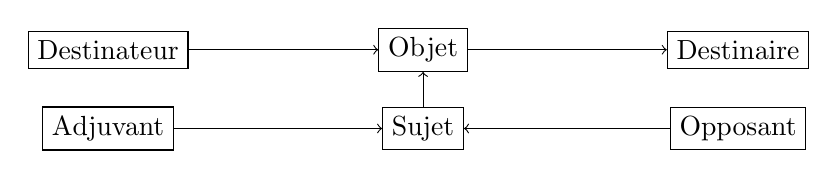
\begin{tikzpicture}
    \node[draw] (P) at (0,0) {Adjuvant};
    \node[draw] (S) at (4,0) {Sujet};
    \node[draw] (Q) at (8,0) {Opposant};
    \draw[->] (P) -- (S);
    \draw[<-] (S) -- (Q);
    \node[draw] (A) at (0,1) {Destinateur};
    \node[draw] (B) at (4,1) {Objet};
    \node[draw] (C) at (8,1) {Destinaire};
    \draw[->] (A) -- (B);
    \draw[->] (B) -- (C);
    \draw[->] (S) -- (B);
  \end{tikzpicture}
  \begin{block}{}
    Chaque couple est relié par une implication et chaque élément du schéma répartit les sphères d'actions de Propp.
  \end{block}
\end{frame}

\begin{frame}{Transition vers une aventure}
  Greimas propose des cas de démarrage de quêtes ($\uparrow$):
  \begin{itemize}
    \item Réalisation réfléchie (absence de médiation)
    \item Réalisation transitive (Action relayée par un tier actant)
    \item Virtualisation réfléchie (Renonciation)
    \item Virtualisation transitivie (Dépossession)
    \item Modèle actantiel mythique (Corrélation avec une structure mythique)
  \end{itemize}
\end{frame}

\subsection{Structures remarquables}
\begin{frame}{Notations phénomènologiques}
  \begin{itemize}
    \item $O vs \bar{O}$ : Distinction du statut du héros (Quêteur, sauveur, victime).
    \item $S vs \bar{S}$ : ou dans $S$, le héros sert des intérêts communs, dans $\bar{S}$ le héros sert des intérêts d'un tierce+.
    \item $F vs \bar{F}$ : distinction des collisions familliales.
    \item $M vs \bar{M}$ : Extraction du caracère mythique de l'épreuve fondamentale.
  \end{itemize}
\end{frame}

\begin{frame}{Types fondamentaux}
  \begin{itemize}
    \item $O\bar{S}\bar{F}M$ : Conte héroïque de type \textbf{Quête}
    \item $\bar{O}S\bar{F}M$ : Conte archaïques \textbf{(Le petit poucet)}
    \item etc. En jouant sur les oppositions, on peut isoler des types fondamentaux de contes.
  \end{itemize}
\end{frame}

\section{Implémentation}
\subsection{Représentation d'une quête (statique)}
\begin{frame}{Structure de représentation d'une quête}
  \begin{itemize}
  \item  Etiquette fonctionnelle (Propp)
    \item Implication sur l'histoire (collection de quêtes)
    \item Opération de chainage des quêtes, d'insertion
    \item Opération de transformation des quêtes
    \end{itemize}
\end{frame}

\subsection{La quête comme une monade}
\begin{frame}{La quête comme une monade}
  \begin{itemize}
  \item  Constitué d'une information (décoration) d'état
  \item Combinable (et potentiellement neutre)
  \item Chainable (succession chronologique des quêtes)
  \end{itemize}
Chainage par continuation
\end{frame}

\section{FIN ,Merci. Des questions?}
\subsection{Bibliographie}
\begin{frame}{Bibliographie}
  \scriptsize
  \begin{itemize}
    \item \textbf{Propp Vladimir} "Morphologie du conte",\newline Paris, Seuil, 1970
    \item \textbf{Propp Vladimir} "La transformation des contes merveilleux",\newline Paris, Seuil, 1970
    \item \textbf{Montalbetti Christine} "Le personnage",\newline Paris, Flamarion, 2003
    \item \textbf{Todorov Tzvetan} "Théorie de la littérature",\newline Paris, Seuil, 2001
    \item \textbf{Barthes Roland} "L'aventure sémiologique",\newline Paris, Seuil, 1985
    \item \textbf{MBala Ze Barnabé} "Algirdas Julien Greimas et la science des signes",\newline Cameroun, L'Harmattan, 2012
    \item \textbf{de Saussure Ferdinand} "Cours de Linguistique générale",\newline Paris, Payot, 1967
  \end{itemize}
\end{frame}

\begin{frame}{Complément bibliographiques}
  \begin{block}{A propos de Levi-Strauss}
    L'oeuvre de Levi-Strauss a beaucoup guidé mon travail mais n'est pas usé dans ma présentation (son assertion est développée dans la morphologie du conte), donc je cite quelques un des ouvrages inspirants : 
    \begin{itemize}
      \item La Quadrilogie Mythologie.
      \item Anthropologie Structurale.
      \item Tristes tropiques
      \item La pensée sauvage
    \end{itemize}
  \end{block}
  
\end{frame}





\end{document}